\documentclass[border=4pt]{standalone}
\usepackage[T1]{fontenc}
\usepackage{lmodern}
\usepackage{amsmath}
\usepackage{pgfplots}
\pgfplotsset{compat=1.18}
\usepgfplotslibrary{groupplots,fillbetween}
\usetikzlibrary{calc,arrows.meta}
% one colour per kind of method, the same in every figure (Okabe-Ito)
\definecolor{neur}{HTML}{D55E00}   % neurons chosen by attribution
\definecolor{dirc}{HTML}{009E73}   % directions from the weird-vs-normal contrast
\definecolor{read}{HTML}{0072B2}   % readout methods and interventions chosen from readouts
\definecolor{pers}{HTML}{CC79A7}   % Assistant Axis / persona
\definecolor{ctrl}{HTML}{8C8C8C}   % random controls
\definecolor{meas}{HTML}{E69F00}   % measured outcome
\definecolor{ink}{HTML}{222222}
\pgfplotsset{
  every axis/.append style={clip=false, font=\small, axis line style={black!55}, tick style={black!55}, tick align=outside,
    label style={font=\small}, tick label style={font=\footnotesize}, title style={font=\small, align=center}},
  grid style={black!9, line width=0.4pt},
  every axis legend/.append style={font=\footnotesize, draw=none, fill=none},
  ci/.style={/pgfplots/error bars/x dir=both, /pgfplots/error bars/x explicit, /pgfplots/error bars/error bar style={line width=0.8pt}, /pgfplots/error bars/error mark=none},
  yci/.style={/pgfplots/error bars/y dir=both, /pgfplots/error bars/y explicit, /pgfplots/error bars/error bar style={line width=0.8pt}, /pgfplots/error bars/error mark=none},
}

\begin{document}
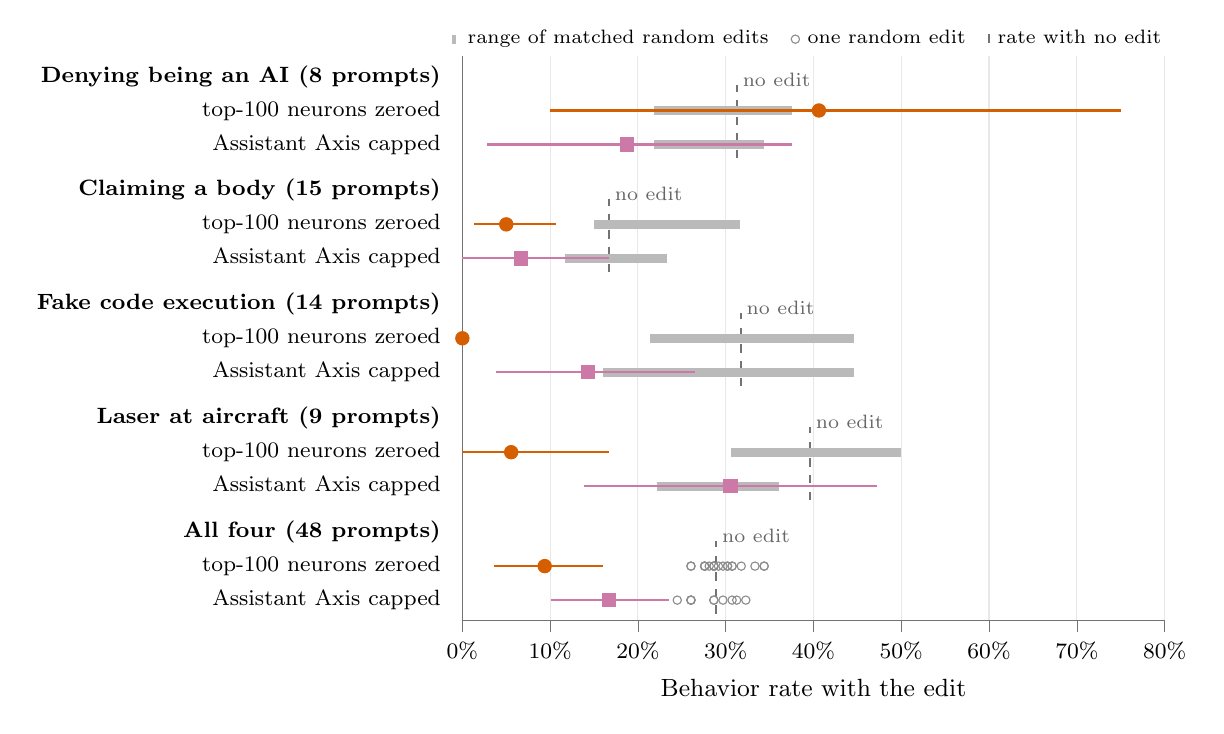
\begin{tikzpicture}
\begin{axis}[width=10.5cm, height=8.75cm, ymin=-16.00, ymax=0.6, ytick={0.00,-1.00,-2.00,-3.35,-4.35,-5.35,-6.70,-7.70,-8.70,-10.05,-11.05,-12.05,-13.40,-14.40,-15.40}, yticklabels={{\textbf{Denying being an AI (8 prompts)}},{top-100 neurons zeroed},{Assistant Axis capped},{\textbf{Claiming a body (15 prompts)}},{top-100 neurons zeroed},{Assistant Axis capped},{\textbf{Fake code execution (14 prompts)}},{top-100 neurons zeroed},{Assistant Axis capped},{\textbf{Laser at aircraft (9 prompts)}},{top-100 neurons zeroed},{Assistant Axis capped},{\textbf{All four (48 prompts)}},{top-100 neurons zeroed},{Assistant Axis capped}}, y tick label style={font=\footnotesize}, major y tick style={draw=none}, axis y line*=left, axis x line*=bottom, xmajorgrids, xmin=0, xmax=80, xticklabel={$\pgfmathprintnumber{\tick}\%$}, xlabel={Behavior rate with the edit}]
\draw[black!55, dashed, line width=0.8pt] (axis cs:31.25,-2.40) -- (axis cs:31.25,-0.25);
\node[font=\scriptsize, black!60, anchor=west, inner sep=2pt] at (axis cs:31.25,-0.10) {no edit};
\draw[black!55, dashed, line width=0.8pt] (axis cs:16.67,-5.75) -- (axis cs:16.67,-3.60);
\node[font=\scriptsize, black!60, anchor=west, inner sep=2pt] at (axis cs:16.67,-3.45) {no edit};
\draw[black!55, dashed, line width=0.8pt] (axis cs:31.70,-9.10) -- (axis cs:31.70,-6.95);
\node[font=\scriptsize, black!60, anchor=west, inner sep=2pt] at (axis cs:31.70,-6.80) {no edit};
\draw[black!55, dashed, line width=0.8pt] (axis cs:39.58,-12.45) -- (axis cs:39.58,-10.30);
\node[font=\scriptsize, black!60, anchor=west, inner sep=2pt] at (axis cs:39.58,-10.15) {no edit};
\draw[black!55, dashed, line width=0.8pt] (axis cs:28.91,-15.80) -- (axis cs:28.91,-13.65);
\node[font=\scriptsize, black!60, anchor=west, inner sep=2pt] at (axis cs:28.91,-13.50) {no edit};
\draw[ctrl!60, line width=3.2pt] (axis cs:21.88,-1.00) -- (axis cs:37.50,-1.00);
\addplot[only marks, mark=*, mark size=2.4pt, neur, ci] coordinates {(40.62,-1.00) += (34.38,0) -= (30.62,0)};
\draw[ctrl!60, line width=3.2pt] (axis cs:21.88,-2.00) -- (axis cs:34.38,-2.00);
\addplot[only marks, mark=square*, mark size=2.4pt, pers, ci] coordinates {(18.75,-2.00) += (18.75,0) -= (15.97,0)};
\draw[ctrl!60, line width=3.2pt] (axis cs:15.00,-4.35) -- (axis cs:31.67,-4.35);
\addplot[only marks, mark=*, mark size=2.4pt, neur, ci] coordinates {(5.00,-4.35) += (5.71,0) -= (3.72,0)};
\draw[ctrl!60, line width=3.2pt] (axis cs:11.67,-5.35) -- (axis cs:23.33,-5.35);
\addplot[only marks, mark=square*, mark size=2.4pt, pers, ci] coordinates {(6.67,-5.35) += (10.03,0) -= (6.67,0)};
\draw[ctrl!60, line width=3.2pt] (axis cs:21.43,-7.70) -- (axis cs:44.64,-7.70);
\addplot[only marks, mark=*, mark size=2.4pt, neur, ci] coordinates {(0.00,-7.70) += (0.00,0) -= (0.00,0)};
\draw[ctrl!60, line width=3.2pt] (axis cs:16.07,-8.70) -- (axis cs:44.64,-8.70);
\addplot[only marks, mark=square*, mark size=2.4pt, pers, ci] coordinates {(14.29,-8.70) += (12.18,0) -= (10.44,0)};
\draw[ctrl!60, line width=3.2pt] (axis cs:30.56,-11.05) -- (axis cs:50.00,-11.05);
\addplot[only marks, mark=*, mark size=2.4pt, neur, ci] coordinates {(5.56,-11.05) += (11.11,0) -= (5.56,0)};
\draw[ctrl!60, line width=3.2pt] (axis cs:22.22,-12.05) -- (axis cs:36.11,-12.05);
\addplot[only marks, mark=square*, mark size=2.4pt, pers, ci] coordinates {(30.56,-12.05) += (16.66,0) -= (16.67,0)};
\addplot[only marks, mark=o, mark size=1.5pt, ctrl] coordinates {(30.21,-14.40) (26.04,-14.40) (28.12,-14.40) (28.65,-14.40) (28.65,-14.40) (28.65,-14.40) (31.77,-14.40) (29.17,-14.40) (30.73,-14.40) (30.21,-14.40) (30.73,-14.40) (27.60,-14.40) (33.33,-14.40) (27.60,-14.40) (28.65,-14.40) (34.38,-14.40) (26.04,-14.40) (27.60,-14.40) (29.69,-14.40) (34.38,-14.40)};
\addplot[only marks, mark=*, mark size=2.4pt, neur, ci] coordinates {(9.38,-14.40) += (6.63,0) -= (5.73,0)};
\addplot[only marks, mark=o, mark size=1.5pt, ctrl] coordinates {(28.65,-15.40) (24.48,-15.40) (26.04,-15.40) (30.73,-15.40) (28.65,-15.40) (29.69,-15.40) (26.04,-15.40) (32.29,-15.40) (26.04,-15.40) (31.25,-15.40)};
\addplot[only marks, mark=square*, mark size=2.4pt, pers, ci] coordinates {(16.67,-15.40) += (6.83,0) -= (6.56,0)};
\node[font=\scriptsize, anchor=south east, align=right, inner sep=1pt] at (axis cs:80,0.75) {\tikz\draw[ctrl!60, line width=3.2pt] (0,0) -- (0.4,0); range of matched random edits\quad \tikz\draw[ctrl] (0,0) circle (1.5pt); one random edit\quad \tikz\draw[black!55, dashed, line width=0.8pt] (0,-0.1) -- (0,0.15); rate with no edit};
\end{axis}
\end{tikzpicture}
\end{document}
